\section{Saules paneļi}
\begin{table}[h]
    \caption{JA tipa paneļu saražotā enerģija uz kvadrātmetru}
    \begin{center}
    %%%%%%%%%%%%%%%%%%%%%%%%%%%%%%%%%%%%%%%%%%%%%%%%%%%%%%%%%%%%%%%%%%%%%%
%%                                                                  %%
%%  This is a LaTeX2e table fragment exported from Gnumeric.        %%
%%                                                                  %%
%%%%%%%%%%%%%%%%%%%%%%%%%%%%%%%%%%%%%%%%%%%%%%%%%%%%%%%%%%%%%%%%%%%%%%
\begin{tabular}{ | c | r r r r r r | } \hline
E, $\textrm{Whm}^{-2}$	&A.13	&R.13	&D.13	&D.40	&D.90	&meteo\\ \hline
jan		&346.66	&227.28	&716.37	&2461.00	&2802.04	&12138.68\\
feb		&3198.12	&2742.33	&4266.63	&6448.71	&5989.95	&25142.93\\
mar		&8222.23	&7397.80	&9472.24	&11938.03	&8717.90	&61764.12\\
apr		&19886.40	&19230.18	&23268.02	&25425.75	&18249.96	&141410.71\\ \hline
$\textrm{E_{sum}}$, $\textrm{kWhm}^{-2}$	&31.7	&29.6	&37.7	&46.3	&35.8	&240.5\\ \hline
\end{tabular}
    \end{center}
    \label{tab:JA}
\end{table}

\begin{table}[h]
    \caption{JA tipa paneļu efektivitāte}
    \begin{center}
    %%%%%%%%%%%%%%%%%%%%%%%%%%%%%%%%%%%%%%%%%%%%%%%%%%%%%%%%%%%%%%%%%%%%%%
%%                                                                  %%
%%  This is a LaTeX2e table fragment exported from Gnumeric.        %%
%%                                                                  %%
%%%%%%%%%%%%%%%%%%%%%%%%%%%%%%%%%%%%%%%%%%%%%%%%%%%%%%%%%%%%%%%%%%%%%%
\begin{tabular}{ | c | c c c c c | }\hline
E	&A.13	&R.13	&D.13	&D.40	&D.90\\ \hline
jan		&0.03	&0.02	&0.06	&0.20	&0.23\\
feb		&0.13	&0.11	&0.17	&0.26	&0.24\\
mar		&0.13	&0.12	&0.15	&0.19	&0.14\\
apr		&0.14	&0.14	&0.16	&0.18	&0.13\\ \hline
vid		&0.11	&0.10	&0.14	&0.21	&0.18\\ \hline
\end{tabular}
    \end{center}
    \label{tab:JA_eff}
\end{table}

\begin{table}[h]
    \caption{JA tipa paneļu efektivitāte procentos}
    \begin{center}
    %%%%%%%%%%%%%%%%%%%%%%%%%%%%%%%%%%%%%%%%%%%%%%%%%%%%%%%%%%%%%%%%%%%%%%
%%                                                                  %%
%%  This is a LaTeX2e table fragment exported from Gnumeric.        %%
%%                                                                  %%
%%%%%%%%%%%%%%%%%%%%%%%%%%%%%%%%%%%%%%%%%%%%%%%%%%%%%%%%%%%%%%%%%%%%%%
\begin{tabular}{ | c | c c c c c | } \hline
E, $\%$	&A.13	&R.13	&D.13	&D.40	&D.90\\ \hline
jan	&2.86	&1.87		&5.90	&20.27	&23.08\\
feb	&12.72	&10.91		&16.97	&25.65	&23.82\\
mar	&13.31	&11.98		&15.34	&19.33	&14.11\\
apr	&14.06	&13.60		&16.45	&17.98	&12.91\\ \hline
vid	&10.74	&9.59		&13.67	&20.81	&18.48\\ \hline
\end{tabular}
    \end{center}
    \label{tab:JA_eff_procenti}
\end{table}

\begin{table}[h]
    \caption{LG tipa paneļu saražotā enerģija uz kvadrātmetru}
    \begin{center}
    %%%%%%%%%%%%%%%%%%%%%%%%%%%%%%%%%%%%%%%%%%%%%%%%%%%%%%%%%%%%%%%%%%%%%%
%%                                                                  %%
%%  This is a LaTeX2e table fragment exported from Gnumeric.        %%
%%                                                                  %%
%%%%%%%%%%%%%%%%%%%%%%%%%%%%%%%%%%%%%%%%%%%%%%%%%%%%%%%%%%%%%%%%%%%%%%
\begin{tabular}{ | c | r r r r r r | }\hline
E, $\textrm{Whm}^{-2}$	&A.13	&R.13	&D.13	&D.40	&D.90	&piranometrs\\ \hline
jan		&495.5	&347.83	&950.75	&2816.81	&3215.06	&12138.68\\
feb		&4431.55	&3625.5	&5046.58	&8253.64	&7413.21	&25142.93\\
mar		&10916.97	&9267.88	&11271.89	&15694.83	&11337.26	&61764.12\\
apr		&27632.28	&25460.2	&29136.2	&34213.52	&23176.05	&141410.71\\ \hline
$E_{sum}$, $\textrm{kWhm}^{-2}$	&43.5	&38.7	&46.4	&70.0		&45.1	&240.5\\ \hline
\end{tabular}
    \end{center}
    \label{tab:LG}
\end{table}

\begin{table}[h]
    \caption{LG tipa paneļu efektivitāte}
    \begin{center}
    %%%%%%%%%%%%%%%%%%%%%%%%%%%%%%%%%%%%%%%%%%%%%%%%%%%%%%%%%%%%%%%%%%%%%%
%%                                                                  %%
%%  This is a LaTeX2e table fragment exported from Gnumeric.        %%
%%                                                                  %%
%%%%%%%%%%%%%%%%%%%%%%%%%%%%%%%%%%%%%%%%%%%%%%%%%%%%%%%%%%%%%%%%%%%%%%
\begin{tabular}{ | c | c c c c c | }\hline
E	&A.13	&R.13	&D.13	&D.40	&D.90\\ \hline
jan		&0.04	&0.03	&0.08	&0.23	&0.26\\
feb		&0.18	&0.14	&0.20	&0.33	&0.29\\
mar		&0.18	&0.15	&0.18	&0.25	&0.18\\
apr		&0.20	&0.18	&0.21	&0.24	&0.16\\ \hline
vid		&0.15	&0.13	&0.17	&0.26	&0.23\\ \hline
\end{tabular}
    \end{center}
    \label{tab:LG_eff}
\end{table}

\begin{table}[h]
    \caption{LG tipa paneļu efektivitāte procentos}
    \begin{center}
    %%%%%%%%%%%%%%%%%%%%%%%%%%%%%%%%%%%%%%%%%%%%%%%%%%%%%%%%%%%%%%%%%%%%%%
%%                                                                  %%
%%  This is a LaTeX2e table fragment exported from Gnumeric.        %%
%%                                                                  %%
%%%%%%%%%%%%%%%%%%%%%%%%%%%%%%%%%%%%%%%%%%%%%%%%%%%%%%%%%%%%%%%%%%%%%%
\begin{tabular}{ | c | c c c c c | }\hline
E, $\%$	&A.13	&R.13	&D.13	&D.40	&D.90\\ \hline
jan		&4.1	&2.9	&7.8	&23.2	&26.5\\
feb		&17.6	&14.4	&20.1	&32.8	&29.5\\
mar		&17.7	&15.0	&18.2	&25.4	&18.4\\
apr		&19.5	&18.0	&20.6	&24.2	&16.4\\ \hline
vid		&14.7	&12.6	&16.7	&26.4	&22.7\\ \hline
\end{tabular}
    \end{center}
    \label{tab:LG_eff_procenti}
\end{table}


\begin{figure}[h]
    \centering
    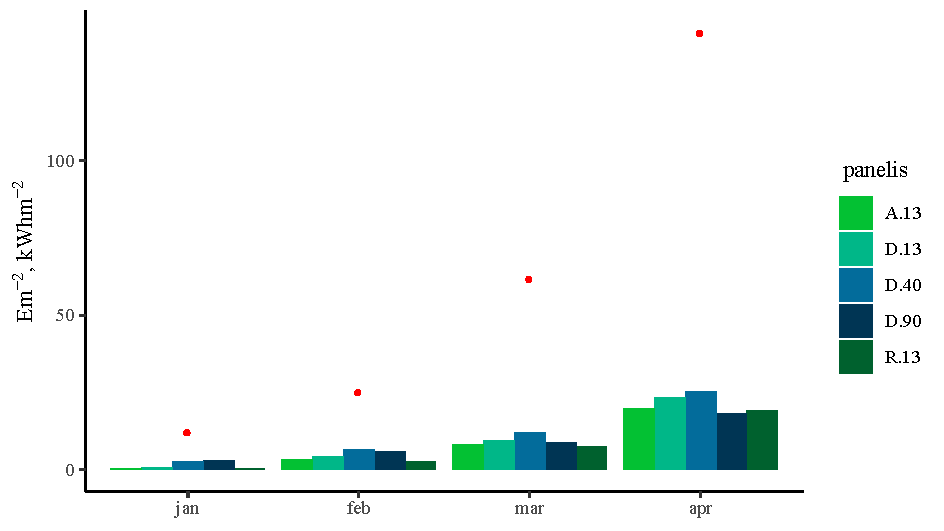
\includegraphics[width=0.6\linewidth]{figures/results/ja_m2.pdf}
    \caption{JA}
    \label{fig:ja}
\end{figure}

% \begin{figure}[h]
%     \centering
%     \includegraphics[width=0.6\linewidth]{figures/results/ja_all_deg.pdf}
%     \caption{JA atkarība no leņķa}
%     \label{fig:ja_deg}
% \end{figure}

% \begin{figure}[h]
%     \centering
%     \includegraphics[width=0.6\linewidth]{figures/results/ja_all_dir.pdf}
%     \caption{JA atkarība no virziena}
%     \label{fig:ja_dir}
% \end{figure}

\begin{figure}[h]
    \centering
    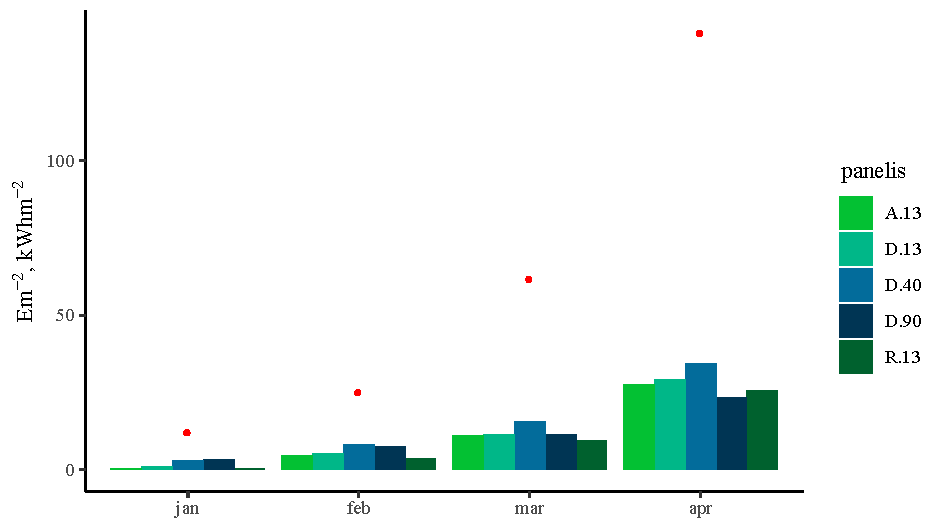
\includegraphics[width=0.6\linewidth]{figures/results/lg_m2.pdf}
    \caption{LG}
    \label{fig:lg}
\end{figure}

\begin{figure}[h]
    \centering
    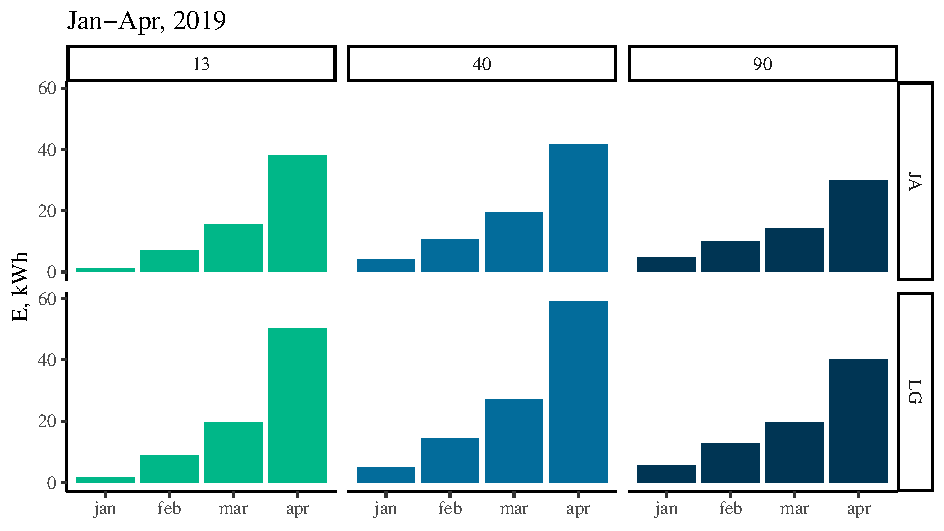
\includegraphics[width=0.6\linewidth]{figures/results/jan_all_deg.pdf}
    \caption{D virziena paneļu atkarība no leņķa}
    \label{fig:ja_deg}
\end{figure}

\begin{figure}[h]
    \centering
    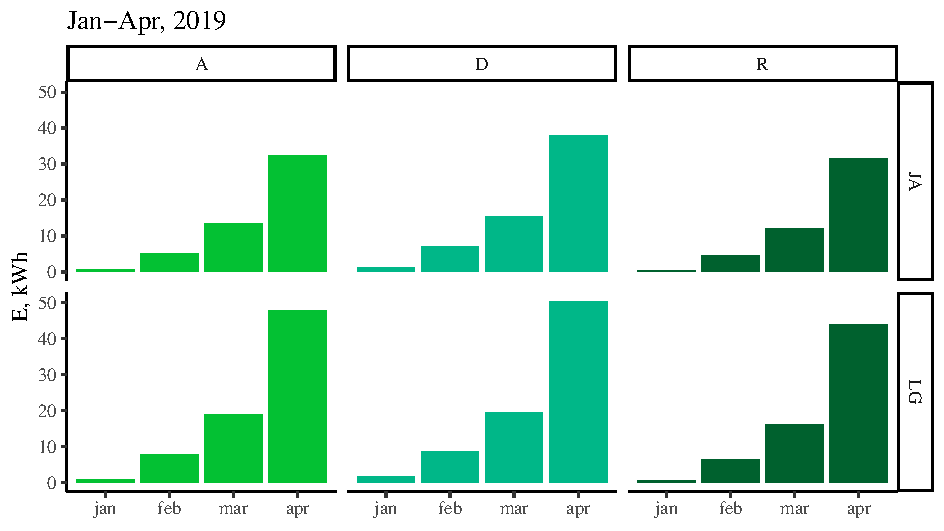
\includegraphics[width=0.6\linewidth]{figures/results/jan_all_dir.pdf}
    \caption{Paneļu ražīguma atkarība no virziena}
    \label{fig:ja_dir}
\end{figure}

\begin{figure}[h]
    \centering
    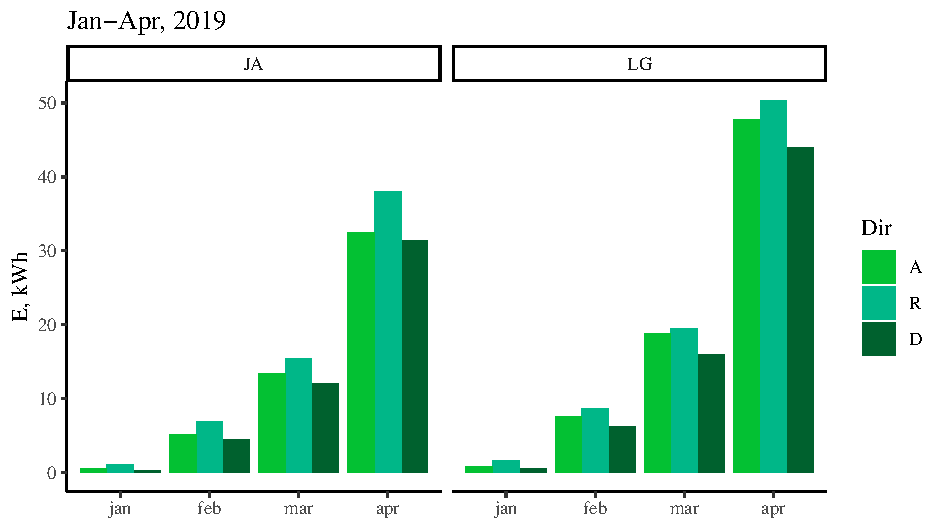
\includegraphics[width=0.6\linewidth]{figures/results/dirType.pdf}
    \caption{JA un LG atkarība no virziena}
    \label{fig:lg_ja_dir}
\end{figure}

\begin{figure}[h]
    \centering
    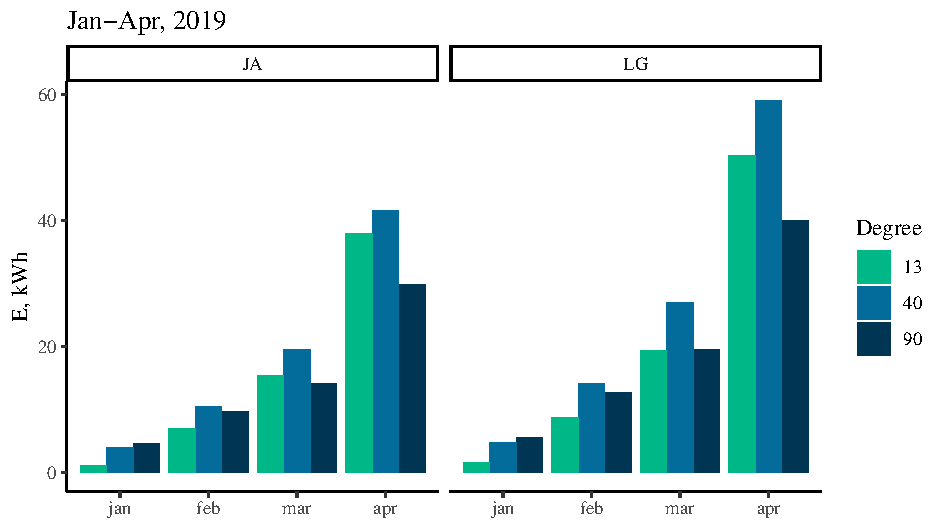
\includegraphics[width=0.6\linewidth]{figures/results/degType.pdf}
    \caption{JA un LG atkarība no leņķa}
    \label{fig:lg_ja_deg}
\end{figure}